\section{温度计}\label{sec:2-3}

\begin{wrapfigure}[30]{r}{6cm}
    \begin{minipage}{2.5cm}
    \centering
    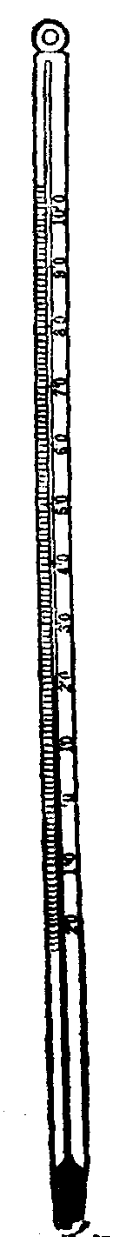
\includegraphics[width=1.5cm]{../pic/czwl2-ch2-9}
    \caption{水银\\温度计}\label{fig:2-9}
    \end{minipage}
    \qquad
    \begin{minipage}{2.5cm}
    \centering
    \vspace{1.8cm}
    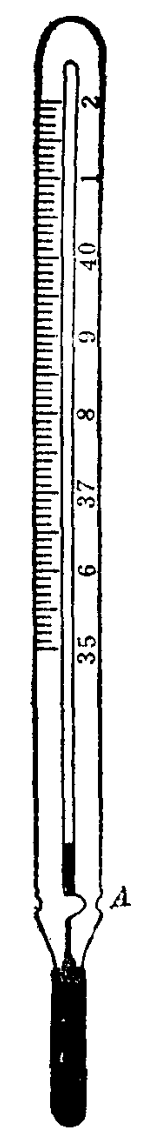
\includegraphics[width=2cm]{../pic/czwl2-ch2-10}
    \caption{体温计}\label{fig:2-10}
    \end{minipage}
\end{wrapfigure}


日常生活中,常用凉、温、烫等词来形容物体的温度。
但是对温度的概念只有这种凭感觉得来的大致的了解,是不够的。
我们要学会准确地测量温度,并且用数值把温度的高低表示出来。
例如,人的正常体温是 37 度,开水的温度是 100 度等。
温度计就是用来测量物体的温度的。

常用的温度计是根据液体热胀冷缩的性质制成的。

实验室里常用的是水银温度计(图 \ref{fig:2-9})。
它的主要部分是一根内径很细而且均匀的玻璃管,管的下端是一个玻璃泡,
在管和泡里有适量的水银,管上标有刻度。
在温度改变时,水银热胀冷缩,管内水银面的位置就随着改变,
从水银达到的刻度就可以读出温度。

常用温度计的刻度,是把冰水混合物的温度规定为 0 度,
把 1 标准气压下的沸水的温度规定为 100 度,
在 0 度和 100 度之间分成 100 等分,每一等分就是 1 度。
这种分度法还可以扩大到 0 度以下和 100 度以上。
用这种办法确定的温度单位叫做\textbf{攝氏度}。
上面提到的人的正常体温和开水的温度,以及日常生活中所说的温度是多少度,都是指摄氏度。

摄氏度用符号 $\celsius$ 来表示。
例如,22 摄氏度就写成 $22\celsius$。
对 $0\celsius$ 以下的温度,还要在度数前边加一个 “$-$” 号。
例如零下 18 摄氏度(或负 18 摄氏度)就写成 $-18\celsius$。

除了水银温度计外,常用的还有酒精温度计、煤油温度计等。
家庭里用来测量气温的温度计,大多是煤油温度计。为了看起来明显,常把煤油染成红色。

温度计不同,测量的范围也不同。
温度计不能用来测量超过它的最高刻度的温度。
因此在使用前应估计被测温度的高低,以免被测温度过高,温度计里的液体把温度计胀破。

温度计能测出物体的温度,是由于温度计的温度能变得与所测物体的温度相同。
因此,使用温度计测量温度时,应使温度计的玻璃泡跟被测物体充分接触。
例如,测量液体的温度时,要使温度计的玻璃泡完全浸没在液体中。
在观察温度计的时候,不要把温度计从液体中拿出来,而应当仍旧放在液体中读数。

医用温度计也叫体温计(图 \ref{fig:2-10}),是用来测量人体温度的。
人体温度的变化一般在 $35\celsius$ 到 $42\celsius$ 之间,
所以体温计的刻度通常是从 $35\celsius$ 到 $42\celsius$。
体温计的泡的容积要比上面的细管的容积大得多,泡里水银的微小膨胀,
就能使细管内水银柱的长度发生显著的变化。
这样就使体温计的测量能准确到十分之一摄氏度。
体温计在 $A$ 点附近管子非常细,水银可以通过这里升到上面去,
温度计离开人体后,水银变冷收缩,水银柱就在这里断开,使上面的水银退不回来。
所以体温计离开人体以后还能表示人体的温度.要使已经升上去的水银再回到泡里,
可以拿着体温计的上部用力往下甩(不是医用的普通温度计不能甩)。

除了上述的液体温度计外,还可以利用物质随温度而改变的其他特性制成其他类型的温度计。


